\graphicspath{{./images/}}

\chapter{Laufzeitsicht}

\section{Ebene 1}

\subsection{Registrierung}

Die Registrierungs Sequence ist ein mehrstufiger Prozess. Hat der neu Händler ein Produkt ausgewählt und seine Daten eingegeben, werden diese in der Datenbank gespeichert. Gleichzeitig wird eine SMS in Form einer MTAN sowie eine Mail mit einem Registierungslink verschickt. Sobald der Händler diese Daten erhalten hat, kann er den Prozess fortführen sobald der MTAN Code verfizifiert wurde. Die Übermittlung der Daten an die Workflow Engine erfolgt asynchron.
\begin{center}
	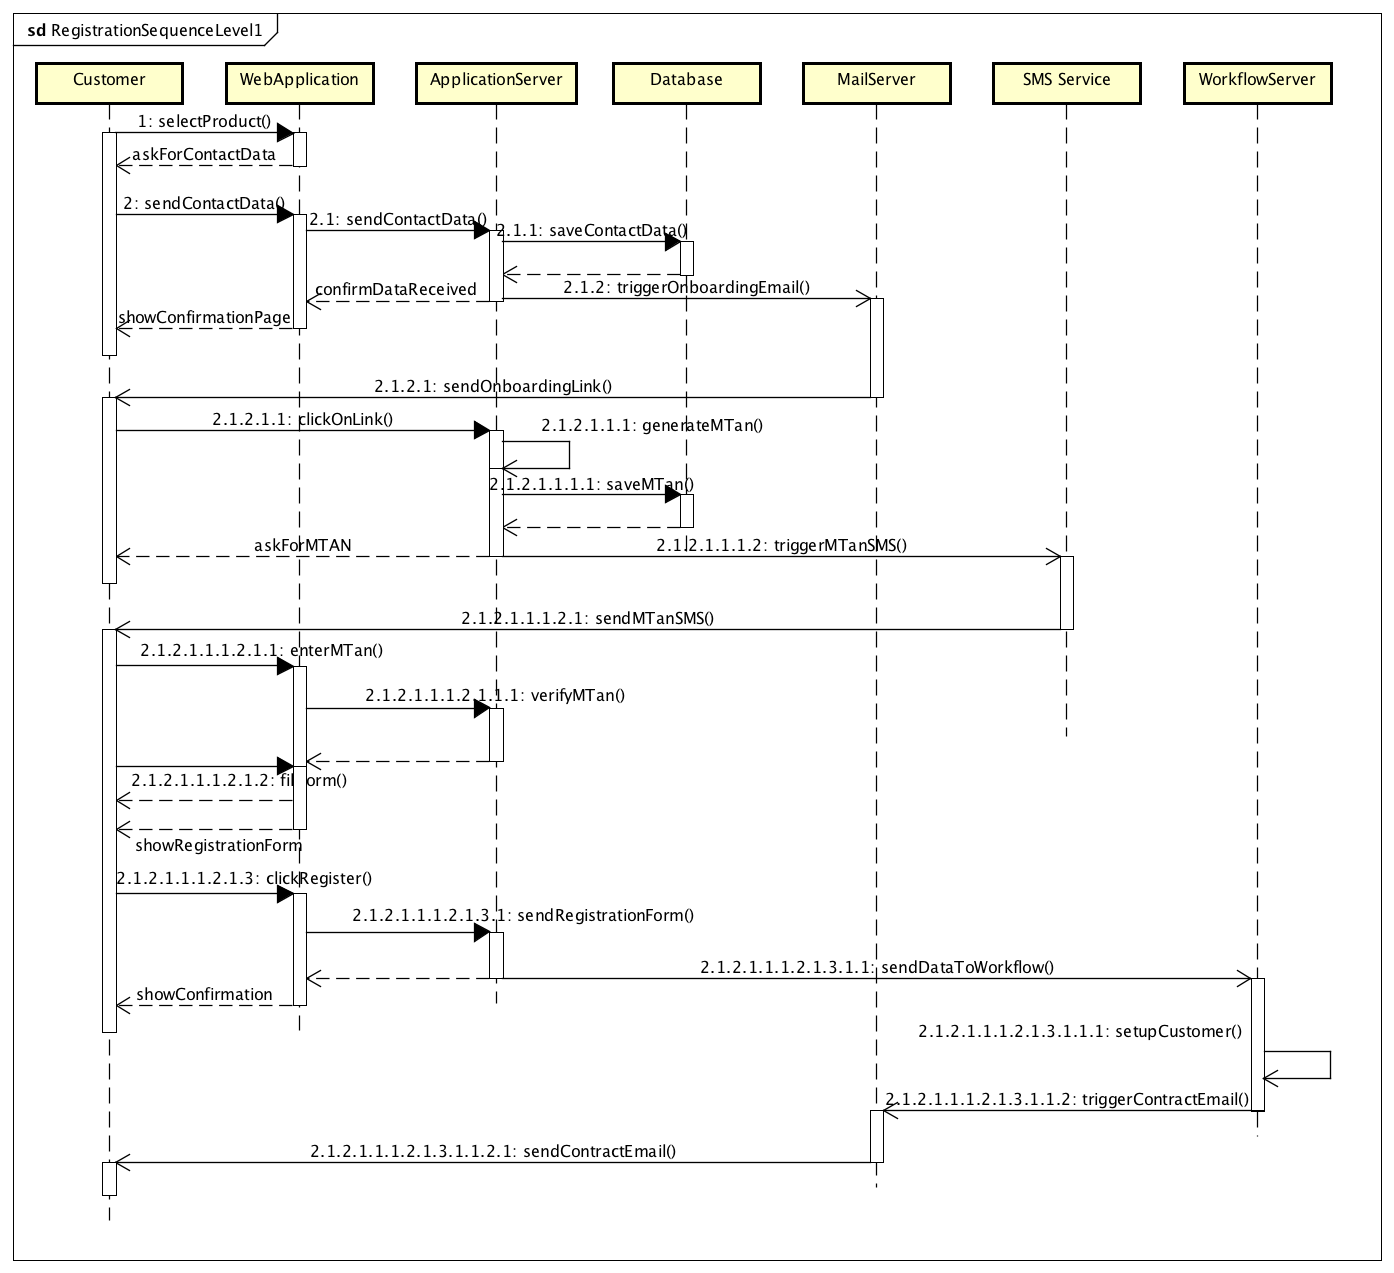
\includegraphics[scale=0.44]{RegistrationSequenceLevel1.png}
\end{center}
\newpage

\subsection{Konfigurationsänderung}

Müssen Properties der Applikation geändert werden, geschiet dies über Dateinen  welche im GIT Repository eingecheckt sind. Über einen Webhook auf dem GIT Server wir über den Config Server eine Nachricht auf die Queue gelegt wodurch die Clients die Properties update können. Spring Cloud Config und Spring Clound Bus stellen alle Funtionen bereits weshalb nur die Konfiguration des Servers, Clients und der Queue gemacht werden muss.
\begin{center}
	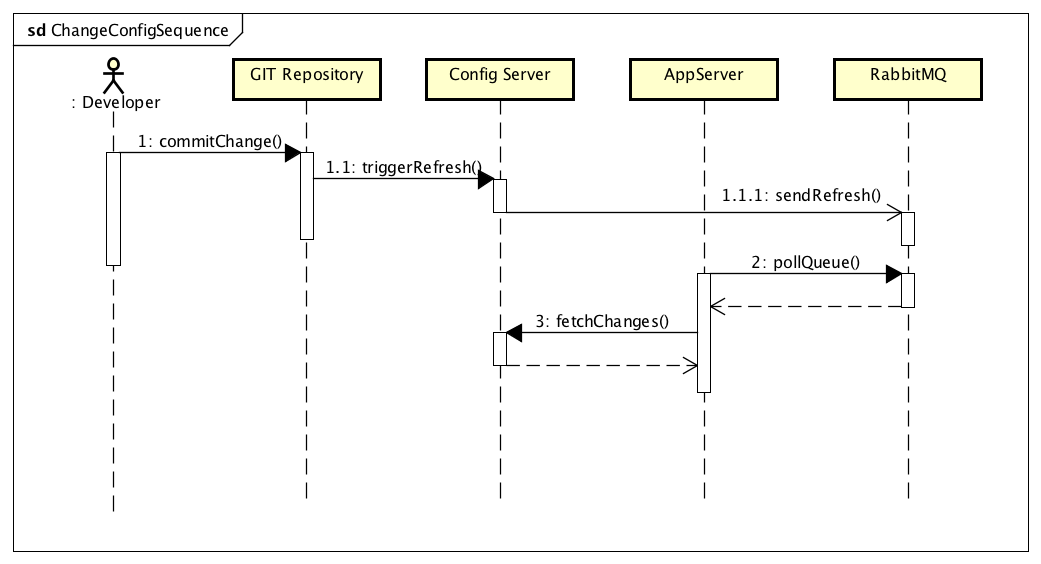
\includegraphics[scale=0.6]{ChangeConfigSequence.png}
\end{center}
\newpage
\section{Ebene 2}

Damit der Prozess der Registierung klarer wird, ist in der folgenden Abbildung der Ablauf detailierter mit den in Kapitel \ref{reg-service} beschriebenen Komponenten dargestellt. Der SchedulerService prüft die Datenbank regelmässig und asynchron zu den Abläufen welcher der RegistrierungsService ausführt. Dadruch wird verhindet, dass der Benutzer im Fall eines Problems mit der Kommunikation der BPM Engine nichts merkt.
\subsection{Registrierung}
\begin{center}
	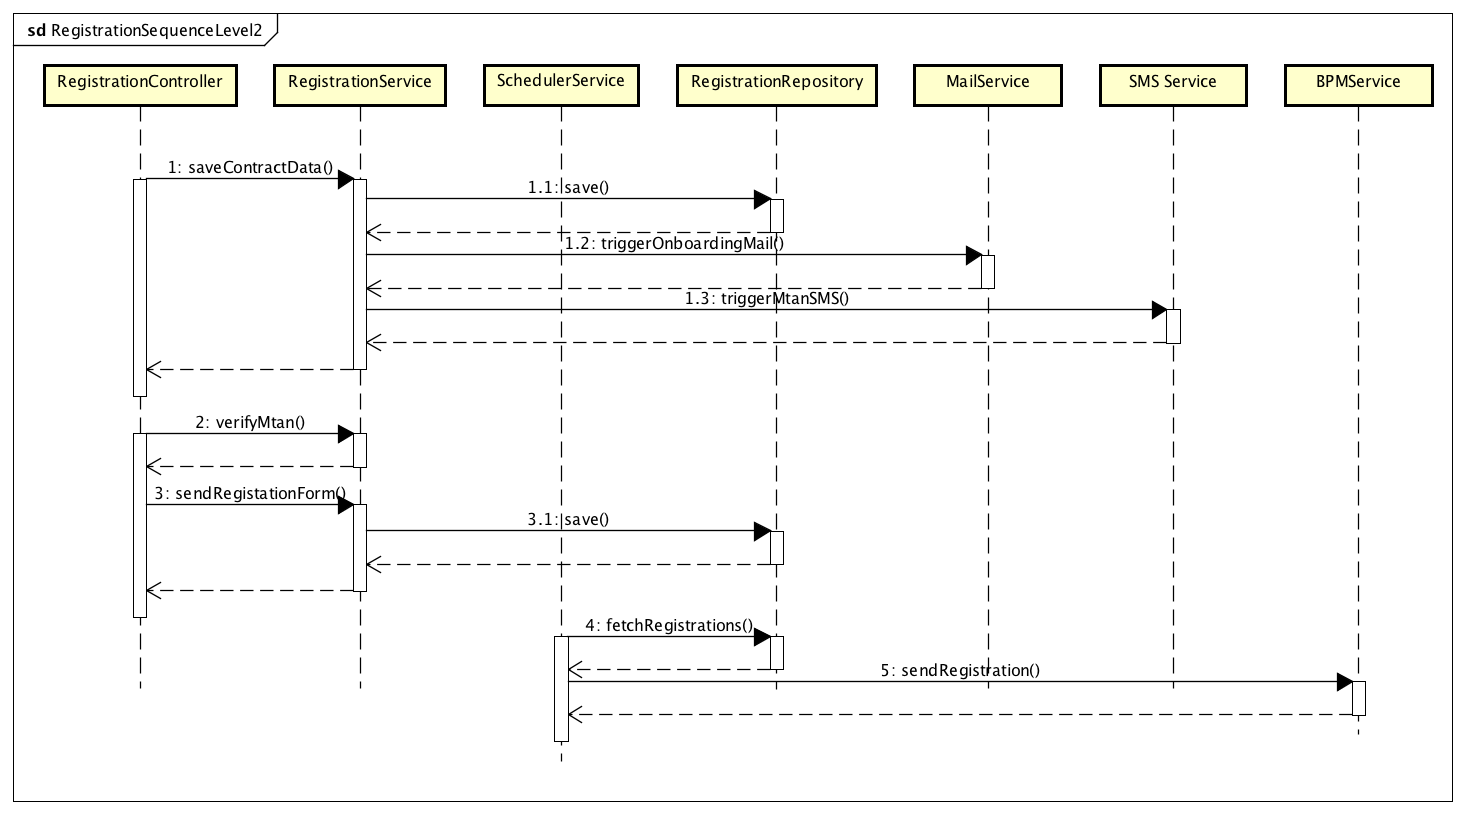
\includegraphics[scale=0.42]{RegistrationSequenceLevel2.png}
\end{center}



